\section{Introduction}

Language-oriented programming (LOP) \cite{LOP} features solving a class of problems by creating new domain-specific languages (DSLs).
To avoid reimplementing common language constructs such as loops and branches,
developers tend to implement DSLs based on another general-purpose programming language (called \textit{host language}).
Developers can define a DSL using language features supported by the host language, rendering programs with domain-specific forms.
Languages with features like macros and higher-order functions are frequently employed as host languages\cite{macro-dsl,macro-dsl-2}.
These features can be treated as methods to implement translations from DSLs to the host language.
By specifying these translation rules, developers can obtain DSL interpreters for free.
This type of DSLs is called embedded DSL (eDSL).

Despite eDSL can significantly reduce implementation efforts, DSL users find it inconvenient because of the inevitable need to learn host language concepts and understand error messages.
This is a type of \textit{abstraction leakage} \cite{Abstraction}:
 the user writes a DSL program which will be translated into the host language,
 causing the executed program is pretty differently from the original program.
It is difficult to access DSL-level information after translation.

Pombrio et al. have made great progress in the maintenance of abstraction automatically for syntactic sugars.
They proposed \textit{resugaring} \cite{resugar}, by selectively reorganizing the sequence of evaluations on the host language to the DSL according to the reverse translation rules.
% In particular, a DSL program is translated into host language first.
% Then, each term in the evaluation sequence of the host language is checked if it can be reconstructed into the DSL constructs dynamically.
However, when the translated program causes an error in the host language,
 the abstraction is still leaked because of the error message,
% However, errors still appear in the host language. %, which cannot be lifted to DSL.
 or DSL users can only observe that the evaluation sequence is stuck, but do not know where the error happens.
Type lifting \cite{infer-types} is another work on maintaining abstraction.
Typing rules for newly-defined language constructs are inferred statically according to the syntactic sugar definitions and the typing rules of the host language.
Then, these inferred typing rules of DSL can guide DSL users, and for example, can be used for static analysis in IDEs.
% and facilitates the generation of high-quality DSL error messages.

Inspired by these work, we expect to lift the semantics of DSL, to overcome drawbacks of resugaring.
The DSL developers only need to provide the translation rules from the DSL to the host language.
We then automatically derive evaluation rules of the DSL constructs based on the semantics of the host language and the translation rules.
We call this \textit{semantics lifting}.
% In other words, for a DSL construct defined by a translation rule, we would like to \textit{derive its evaluation rule}.
The lifted semantics can give the user a better aid in diagnosis when the DSL program is stuck.
It is possible to know, for example, which subexpression causes the error.
We adapt the core ideas of typing rules derivation to semantics lifting.
For example, in a host language with lambda abstraction and application, we can define $\<let>$ by a simple transformation:
\[ \<let>~x:t=e_1~\<in>~e_2 => (λx:t.e_2)~e_1 \]
The evaluation rule derivation of $\<let>$ is given in Fig. \ref{fig:let}.
An expression with $\<let>$ evaluates to $v$ in DSL,
 iff the translated expression evaluates to $v$ in host language (Step 1).
Based on the evaluation rule of application, we can expand the premise (Step 2).
A lambda abstraction is always a value, with no premises (Step 3). 
% And the evaluation rule of lambda abstraction can be applied.
Hence, we can obtain the following evaluation rule for $\<let>$:
\[
  \inference{e_1 \Da v_1 & e_2[v_1/x] \Da v}{\<let>~x:t=e_1~\<in>~e_2 \Da v}
\]
Note that without lambda abstraction and application appearing in the premises,
 the evaluation rule of $\<let>$ is described directly, without referring to host language constructs.
We define the \textit{abstraction} property: evaluation rules of a DSL should be independent of the host language.
And the abstraction property holds in the $\<let>$ case.

\begin{figure}[t!]
  \[
    \inference[(Step 1) ]{%
      \inference[(Step 2) ]{%
        \inference[(Step 3)]{}{%
          λx:t.e_2 \Da λx:t.e_2}
        & e_1 \Da v_1
        & e_2[v_1/x] \Da v
      }
      {(λx:t.e_2)~e_1 \Da v}
    }
    {\<let>~x:t=e_1~\<in>~e_2 \Da v}
  \]
  \caption{Evaluation Rule Derivation of $\mathit{let}$}
  \label{fig:let}
\end{figure}

This approach seems natural. However, after further examination, we are faced with several challenges:
(1) In most cases, it is not possible to statically determine where a lambda abstraction is called,
 and thus it is not possible to statically evaluate the abstraction body.
 When a lambda abstraction is used in a translation rule for a DSL construct definition,
 the evaluation of these host language constructs in the abstraction body is delayed until that lambda abstraction is actually applied at run time.
 Therefore, lambda abstraction with host language constructs may lead to abstraction leakage.
(2) The evaluation rules of applications and let bindings contain the evaluation of substitution in premises, like $e[v/x]$.
 In a concrete derivation, $e$ may be replaced by some compound expression.
 For example, in the derivation of translation rule $e_1~or'~e_2=>\<let>~x:\<bool>=e_1~\<in>~\<if>~x~x~\<false>$, 
  the premises will be $e_1\Da v_1$ and $(\<if>~x~x~e_2)[v_1/x]\Da v$.
For the second premise,
 on the one hand, we need to apply the evaluation rule of $\<if>$ statically for abstraction;
 on the other hand, we need to carefully consider the relationship between the scope of $x$ and sub-expressions like $e_2$ in order to prevent hygiene problem \cite{hygine}.
 Therefore, the derivation with substitution should be stated to maintain abstractness while ensuring correctness.
(3) When deriving rules, we recursively generate premises based on tzhe evaluation rules of language constructs.
 However, the evaluation of many language constructs, like $\<if>$, is defined by multiple rules.
 This may lead to several branches when applying rules in derivation.

To address challenge (1),
 we apply a method similar to \textit{lambda lifting} transformation to translation rules,
 to reveal the body of abstraction \cite{lambda-lifting}.
To address challenge (2),
 we impose strict requirements on translation rules to avoid hygienic problems and ensure correctness,
 and show that applying substitution statically can maintain abstractness.
To address challenge (3),
 we use Skeletal semantics to describe the behaviour of language constructs \cite{skeleton}.
 Each language construct has a unique rule, which facilitates derivation. % guarantees the determinism in derivation.
 We use Skeleton as the meta-language and implement semantic lifting by deriving Skeleton rules for DSL constructs.

By applying techniques above, combined with the existing approach for type lifting,
 developers can define DSLs via translation rules,
 and get the automatically derived evaluation and typing rules of DSLs,
 which maintain abstraction property of DSLs.
At this point, DSLs are host language independent, or standalone.
DSL users are allowed to be fully agnostic of the underlying host language.
Language constructs in the host language that are not expected to be used in the DSL can be safely removed.
We call this \textit{language lifting}, as shown in Fig. \ref{fig:layers}.

\begin{figure}[t]
  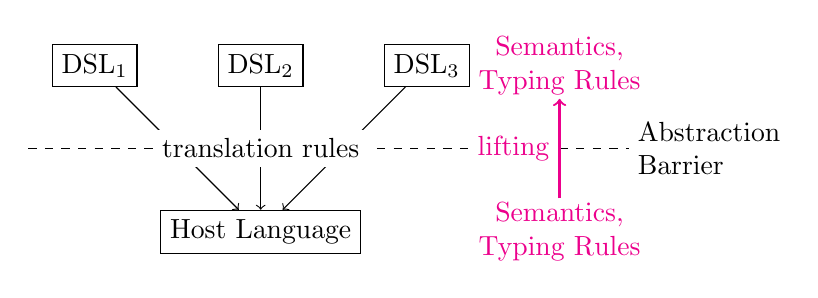
\begin{tikzpicture}[x=6pt,y=6pt,yscale=1,xscale=1]

\draw[dashed] (-14,5) -- (23,5);
\node[align=left,fill=white] at (27,5) {Abstraction\\Barrier};

\node[draw] (H) at (0,0) {Host Language};
\node[draw] (D1) at (-10,10) {DSL$_1$};
\node[draw] (D2) at (0,10) {DSL$_2$};
\node[draw] (D3) at (10,10) {DSL$_3$};

% \node[align=left,text=magenta] (M1) at (14,0) {Semantics, Typing Rules\\of Host Language}; 
\node[align=center,text=magenta] (M1) at (18,0) {Semantics,\\ Typing Rules}; 
\node[align=center,text=magenta] (M2) at (18,10) {Semantics,\\ Typing Rules}; 
 
\draw[->] (D1) -> (H);
\draw[->] (D3) -> (H);
\draw[->] (D2) -> node[fill=white] {translation rules} (H);
% \draw[->,thick,magenta] (9,2) -> node[right=1em] {lifting} (15,8);
\draw[->,thick,magenta] (18,2) -> node[left,fill=white] {lifting} (18,8);

\end{tikzpicture}

  \caption{Language Lifting}
  \label{fig:layers}
\end{figure}

Moreover, the expressiveness of the host language is sometimes insufficient, the absence of some datatypes makes it impossible to define a DSL by translation rules.
To solve this problem, 
 our framework provides meta-extensions (to introduce new primitive operations and datatypes) and monad-extensions (to introduce side effects)
 to extend host language without changing existing semantics.
And to describe the evaluation after monad extensions, we add monad support to the meta-language.
DSL developers can define the DSL constructs via translation rules based on this extended host language now.
We consider this to be a generic DSL design pattern:
 various languages containing different features are extended from the host language,
 and the DSL developers select the appropriately-extended host language and define the DSLs by translation rules.
In this paper, we use simply-typed lambda-calculus (\STLC) as the basic host language.

Our main technical contributions can be summarized as follows:

\begin{itemize}
  % \item We design a meta-language to describe the evaluation rules and typing rules of a language structurally.
  %   % The meta-language can be extended in a modular way.
  %   We formalize the syntax and semantics of our meta-language (Section \ref{sec:meta}).
  %   And then, we define the host language \STLC{} using meta-language (Section \ref{sec:m-host}).
  \item We present a semantics lifting algorithm for DSL constructs defined by translation rules (Section \ref{sec:tr}), and prove the correctness and the abstraction properties of the algorithm.
    % For translation rules defined with lambda abstraction, we illustrate lambda lifting algorithm to maintain abstraction property.
    % Besides, evaluation rules with substitution will not break these properties.
  \item We propose a general DSL implementation workflow, using \STLC{} as the host language:
    first introduce vocabularies by meta-extensions and new language features by monad extensions (Section \ref{sec:ex}),
    then define the DSL constructs by translation rules on the extended language.
    % For each step, we give a formal description with examples.
    % And two strict requirements will be applied to translation rules.
  % \item We present an algorithm to derive evaluation and typing rules for DSL constructs defined by translation rules (Section \ref{sec:alg}).
  %   As major properties of algorithms, we give proofs of correctness and abstraction. 
  %   For translation rules defined with lambda abstraction,
  %    we illustrate lambda lifting method to maintain abstraction property.
  %   Besides, these properties can be guaranteed with substitution in derivation.
  \item We give an implementation of the framework called Osazone (Section \ref{sec:impl}), showcase several case studies as evidence for the power of Osazone (Section \ref{sec:eval}).
\end{itemize}

% Note that the focus of this paper is on the semantics of the language rather than the syntax. 
% Extensions to the syntax, such as parser implementation for DSLs, are not the topic of this paper.
